% Options for packages loaded elsewhere
\PassOptionsToPackage{unicode}{hyperref}
\PassOptionsToPackage{hyphens}{url}
%
\documentclass[
]{article}
\usepackage{amsmath,amssymb}
\usepackage{iftex}
\ifPDFTeX
  \usepackage[T1]{fontenc}
  \usepackage[utf8]{inputenc}
  \usepackage{textcomp} % provide euro and other symbols
\else % if luatex or xetex
  \usepackage{unicode-math} % this also loads fontspec
  \defaultfontfeatures{Scale=MatchLowercase}
  \defaultfontfeatures[\rmfamily]{Ligatures=TeX,Scale=1}
\fi
\usepackage{lmodern}
\ifPDFTeX\else
  % xetex/luatex font selection
\fi
% Use upquote if available, for straight quotes in verbatim environments
\IfFileExists{upquote.sty}{\usepackage{upquote}}{}
\IfFileExists{microtype.sty}{% use microtype if available
  \usepackage[]{microtype}
  \UseMicrotypeSet[protrusion]{basicmath} % disable protrusion for tt fonts
}{}
\makeatletter
\@ifundefined{KOMAClassName}{% if non-KOMA class
  \IfFileExists{parskip.sty}{%
    \usepackage{parskip}
  }{% else
    \setlength{\parindent}{0pt}
    \setlength{\parskip}{6pt plus 2pt minus 1pt}}
}{% if KOMA class
  \KOMAoptions{parskip=half}}
\makeatother
\usepackage{xcolor}
\usepackage[margin=2cm]{geometry}
\usepackage{color}
\usepackage{fancyvrb}
\newcommand{\VerbBar}{|}
\newcommand{\VERB}{\Verb[commandchars=\\\{\}]}
\DefineVerbatimEnvironment{Highlighting}{Verbatim}{commandchars=\\\{\}}
% Add ',fontsize=\small' for more characters per line
\usepackage{framed}
\definecolor{shadecolor}{RGB}{248,248,248}
\newenvironment{Shaded}{\begin{snugshade}}{\end{snugshade}}
\newcommand{\AlertTok}[1]{\textcolor[rgb]{0.94,0.16,0.16}{#1}}
\newcommand{\AnnotationTok}[1]{\textcolor[rgb]{0.56,0.35,0.01}{\textbf{\textit{#1}}}}
\newcommand{\AttributeTok}[1]{\textcolor[rgb]{0.13,0.29,0.53}{#1}}
\newcommand{\BaseNTok}[1]{\textcolor[rgb]{0.00,0.00,0.81}{#1}}
\newcommand{\BuiltInTok}[1]{#1}
\newcommand{\CharTok}[1]{\textcolor[rgb]{0.31,0.60,0.02}{#1}}
\newcommand{\CommentTok}[1]{\textcolor[rgb]{0.56,0.35,0.01}{\textit{#1}}}
\newcommand{\CommentVarTok}[1]{\textcolor[rgb]{0.56,0.35,0.01}{\textbf{\textit{#1}}}}
\newcommand{\ConstantTok}[1]{\textcolor[rgb]{0.56,0.35,0.01}{#1}}
\newcommand{\ControlFlowTok}[1]{\textcolor[rgb]{0.13,0.29,0.53}{\textbf{#1}}}
\newcommand{\DataTypeTok}[1]{\textcolor[rgb]{0.13,0.29,0.53}{#1}}
\newcommand{\DecValTok}[1]{\textcolor[rgb]{0.00,0.00,0.81}{#1}}
\newcommand{\DocumentationTok}[1]{\textcolor[rgb]{0.56,0.35,0.01}{\textbf{\textit{#1}}}}
\newcommand{\ErrorTok}[1]{\textcolor[rgb]{0.64,0.00,0.00}{\textbf{#1}}}
\newcommand{\ExtensionTok}[1]{#1}
\newcommand{\FloatTok}[1]{\textcolor[rgb]{0.00,0.00,0.81}{#1}}
\newcommand{\FunctionTok}[1]{\textcolor[rgb]{0.13,0.29,0.53}{\textbf{#1}}}
\newcommand{\ImportTok}[1]{#1}
\newcommand{\InformationTok}[1]{\textcolor[rgb]{0.56,0.35,0.01}{\textbf{\textit{#1}}}}
\newcommand{\KeywordTok}[1]{\textcolor[rgb]{0.13,0.29,0.53}{\textbf{#1}}}
\newcommand{\NormalTok}[1]{#1}
\newcommand{\OperatorTok}[1]{\textcolor[rgb]{0.81,0.36,0.00}{\textbf{#1}}}
\newcommand{\OtherTok}[1]{\textcolor[rgb]{0.56,0.35,0.01}{#1}}
\newcommand{\PreprocessorTok}[1]{\textcolor[rgb]{0.56,0.35,0.01}{\textit{#1}}}
\newcommand{\RegionMarkerTok}[1]{#1}
\newcommand{\SpecialCharTok}[1]{\textcolor[rgb]{0.81,0.36,0.00}{\textbf{#1}}}
\newcommand{\SpecialStringTok}[1]{\textcolor[rgb]{0.31,0.60,0.02}{#1}}
\newcommand{\StringTok}[1]{\textcolor[rgb]{0.31,0.60,0.02}{#1}}
\newcommand{\VariableTok}[1]{\textcolor[rgb]{0.00,0.00,0.00}{#1}}
\newcommand{\VerbatimStringTok}[1]{\textcolor[rgb]{0.31,0.60,0.02}{#1}}
\newcommand{\WarningTok}[1]{\textcolor[rgb]{0.56,0.35,0.01}{\textbf{\textit{#1}}}}
\usepackage{longtable,booktabs,array}
\usepackage{calc} % for calculating minipage widths
% Correct order of tables after \paragraph or \subparagraph
\usepackage{etoolbox}
\makeatletter
\patchcmd\longtable{\par}{\if@noskipsec\mbox{}\fi\par}{}{}
\makeatother
% Allow footnotes in longtable head/foot
\IfFileExists{footnotehyper.sty}{\usepackage{footnotehyper}}{\usepackage{footnote}}
\makesavenoteenv{longtable}
\usepackage{graphicx}
\makeatletter
\def\maxwidth{\ifdim\Gin@nat@width>\linewidth\linewidth\else\Gin@nat@width\fi}
\def\maxheight{\ifdim\Gin@nat@height>\textheight\textheight\else\Gin@nat@height\fi}
\makeatother
% Scale images if necessary, so that they will not overflow the page
% margins by default, and it is still possible to overwrite the defaults
% using explicit options in \includegraphics[width, height, ...]{}
\setkeys{Gin}{width=\maxwidth,height=\maxheight,keepaspectratio}
% Set default figure placement to htbp
\makeatletter
\def\fps@figure{htbp}
\makeatother
\setlength{\emergencystretch}{3em} % prevent overfull lines
\providecommand{\tightlist}{%
  \setlength{\itemsep}{0pt}\setlength{\parskip}{0pt}}
\setcounter{secnumdepth}{-\maxdimen} % remove section numbering
\ifLuaTeX
  \usepackage{selnolig}  % disable illegal ligatures
\fi
\IfFileExists{bookmark.sty}{\usepackage{bookmark}}{\usepackage{hyperref}}
\IfFileExists{xurl.sty}{\usepackage{xurl}}{} % add URL line breaks if available
\urlstyle{same}
\hypersetup{
  pdftitle={HW1},
  hidelinks,
  pdfcreator={LaTeX via pandoc}}

\title{HW1}
\author{}
\date{\vspace{-2.5em}}

\begin{document}
\maketitle

\hypertarget{question-1}{%
\subsection{Question 1}\label{question-1}}

\hypertarget{b}{%
\paragraph{(b)}\label{b}}

\begin{Shaded}
\begin{Highlighting}[]
\NormalTok{k1 }\OtherTok{=} \DecValTok{600}
\NormalTok{k2 }\OtherTok{=} \DecValTok{300}
\NormalTok{rho\_1 }\OtherTok{=} \FloatTok{0.2}
\NormalTok{rho\_2 }\OtherTok{=} \FloatTok{0.5}
\NormalTok{rho\_3 }\OtherTok{=} \FloatTok{0.8}
\NormalTok{rho }\OtherTok{=} \FunctionTok{c}\NormalTok{(rho\_1, rho\_2, rho\_3)}
\NormalTok{V\_a }\OtherTok{=} \FunctionTok{c}\NormalTok{(}\DecValTok{1}\NormalTok{, }\DecValTok{1}\NormalTok{, }\DecValTok{1}\NormalTok{)}\SpecialCharTok{*}\DecValTok{4}\SpecialCharTok{/}\NormalTok{k1}
\NormalTok{V\_b }\OtherTok{=} \FunctionTok{c}\NormalTok{(}\DecValTok{1}\NormalTok{, }\DecValTok{1}\NormalTok{, }\DecValTok{1}\NormalTok{)}\SpecialCharTok{*}\DecValTok{8}\SpecialCharTok{*}\NormalTok{(}\DecValTok{1}\SpecialCharTok{{-}}\NormalTok{rho)}\SpecialCharTok{/}\NormalTok{k2}
\NormalTok{V\_c }\OtherTok{=} \FunctionTok{c}\NormalTok{(}\DecValTok{1}\NormalTok{, }\DecValTok{1}\NormalTok{, }\DecValTok{1}\NormalTok{)}\SpecialCharTok{*}\DecValTok{2}\SpecialCharTok{*}\NormalTok{(}\DecValTok{1}\SpecialCharTok{{-}}\NormalTok{rho)}\SpecialCharTok{/}\NormalTok{k2}
\NormalTok{V\_d }\OtherTok{=} \FunctionTok{c}\NormalTok{(}\DecValTok{1}\NormalTok{, }\DecValTok{1}\NormalTok{, }\DecValTok{1}\NormalTok{)}\SpecialCharTok{*}\DecValTok{2}\SpecialCharTok{*}\NormalTok{(rho}\SpecialCharTok{+}\DecValTok{1}\NormalTok{)}\SpecialCharTok{/}\NormalTok{k2}
\NormalTok{b  }\OtherTok{=} \FunctionTok{cbind}\NormalTok{(rho, V\_a, V\_b, V\_c, V\_d) }\SpecialCharTok{\%\textgreater{}\%} \FunctionTok{as.data.frame}\NormalTok{()}
\FunctionTok{options}\NormalTok{(}\AttributeTok{digits =} \DecValTok{2}\NormalTok{)}
\FunctionTok{print}\NormalTok{(b)}
\end{Highlighting}
\end{Shaded}

\begin{verbatim}
##   rho    V_a    V_b    V_c   V_d
## 1 0.2 0.0067 0.0213 0.0053 0.008
## 2 0.5 0.0067 0.0133 0.0033 0.010
## 3 0.8 0.0067 0.0053 0.0013 0.012
\end{verbatim}

For minimum variance, for any \(\rho\), I would always choose Crossover
study to minimize uncertainty.

\hypertarget{c}{%
\paragraph{(c)}\label{c}}

\begin{Shaded}
\begin{Highlighting}[]
\NormalTok{k1 }\OtherTok{=} \DecValTok{600}
\NormalTok{k2 }\OtherTok{=} \DecValTok{400}
\NormalTok{rho\_1 }\OtherTok{=} \FloatTok{0.2}
\NormalTok{rho\_2 }\OtherTok{=} \FloatTok{0.5}
\NormalTok{rho\_3 }\OtherTok{=} \FloatTok{0.8}
\NormalTok{rho }\OtherTok{=} \FunctionTok{c}\NormalTok{(rho\_1, rho\_2, rho\_3)}
\NormalTok{V\_a }\OtherTok{=} \FunctionTok{c}\NormalTok{(}\DecValTok{1}\NormalTok{, }\DecValTok{1}\NormalTok{, }\DecValTok{1}\NormalTok{)}\SpecialCharTok{*}\DecValTok{4}\SpecialCharTok{/}\NormalTok{k1}
\NormalTok{V\_b }\OtherTok{=} \FunctionTok{c}\NormalTok{(}\DecValTok{1}\NormalTok{, }\DecValTok{1}\NormalTok{, }\DecValTok{1}\NormalTok{)}\SpecialCharTok{*}\DecValTok{8}\SpecialCharTok{*}\NormalTok{(}\DecValTok{1}\SpecialCharTok{{-}}\NormalTok{rho)}\SpecialCharTok{/}\NormalTok{k2}
\NormalTok{V\_c }\OtherTok{=} \FunctionTok{c}\NormalTok{(}\DecValTok{1}\NormalTok{, }\DecValTok{1}\NormalTok{, }\DecValTok{1}\NormalTok{)}\SpecialCharTok{*}\DecValTok{2}\SpecialCharTok{*}\NormalTok{(}\DecValTok{1}\SpecialCharTok{{-}}\NormalTok{rho)}\SpecialCharTok{/}\NormalTok{k2}
\NormalTok{V\_d }\OtherTok{=} \FunctionTok{c}\NormalTok{(}\DecValTok{1}\NormalTok{, }\DecValTok{1}\NormalTok{, }\DecValTok{1}\NormalTok{)}\SpecialCharTok{*}\DecValTok{2}\SpecialCharTok{*}\NormalTok{(rho}\SpecialCharTok{+}\DecValTok{1}\NormalTok{)}\SpecialCharTok{/}\NormalTok{k2}
\NormalTok{c  }\OtherTok{=} \FunctionTok{cbind}\NormalTok{(rho, V\_a, V\_b, V\_c, V\_d) }\SpecialCharTok{\%\textgreater{}\%} \FunctionTok{as.data.frame}\NormalTok{()}
\FunctionTok{options}\NormalTok{(}\AttributeTok{digits =} \DecValTok{2}\NormalTok{)}
\FunctionTok{print}\NormalTok{(c)}
\end{Highlighting}
\end{Shaded}

\begin{verbatim}
##   rho    V_a   V_b    V_c    V_d
## 1 0.2 0.0067 0.016 0.0040 0.0060
## 2 0.5 0.0067 0.010 0.0025 0.0075
## 3 0.8 0.0067 0.004 0.0010 0.0090
\end{verbatim}

For minimum variance, for any \(\rho\), I would always choose Crossover
study to minimize uncertainty.

\begin{Shaded}
\begin{Highlighting}[]
\FunctionTok{load}\NormalTok{(}\StringTok{"\textasciitilde{}/Documents/2023Fall/P8157/P8157/Six Cities.RData"}\NormalTok{)}
\CommentTok{\# data summmary}
\FunctionTok{nrow}\NormalTok{(topeka)}
\end{Highlighting}
\end{Shaded}

\begin{verbatim}
## [1] 1994
\end{verbatim}

\begin{Shaded}
\begin{Highlighting}[]
\FunctionTok{length}\NormalTok{(}\FunctionTok{unique}\NormalTok{(topeka}\SpecialCharTok{$}\NormalTok{id))}
\end{Highlighting}
\end{Shaded}

\begin{verbatim}
## [1] 300
\end{verbatim}

\begin{Shaded}
\begin{Highlighting}[]
\NormalTok{visit }\OtherTok{=}\NormalTok{ topeka }\SpecialCharTok{\%\textgreater{}\%} \FunctionTok{group\_by}\NormalTok{(id) }\SpecialCharTok{\%\textgreater{}\%}\FunctionTok{tally}\NormalTok{()}
\FunctionTok{summary}\NormalTok{(visit}\SpecialCharTok{$}\NormalTok{n)}
\end{Highlighting}
\end{Shaded}

\begin{verbatim}
##    Min. 1st Qu.  Median    Mean 3rd Qu.    Max. 
##     1.0     3.0     7.0     6.6    10.0    12.0
\end{verbatim}

\begin{Shaded}
\begin{Highlighting}[]
\NormalTok{skimr}\SpecialCharTok{::}\FunctionTok{skim}\NormalTok{(topeka)}
\end{Highlighting}
\end{Shaded}

\begin{longtable}[]{@{}ll@{}}
\caption{Data summary}\tabularnewline
\toprule\noalign{}
\endfirsthead
\endhead
\bottomrule\noalign{}
\endlastfoot
Name & topeka \\
Number of rows & 1994 \\
Number of columns & 6 \\
\_\_\_\_\_\_\_\_\_\_\_\_\_\_\_\_\_\_\_\_\_\_\_ & \\
Column type frequency: & \\
numeric & 6 \\
\_\_\_\_\_\_\_\_\_\_\_\_\_\_\_\_\_\_\_\_\_\_\_\_ & \\
Group variables & None \\
\end{longtable}

\textbf{Variable type: numeric}

\begin{longtable}[]{@{}
  >{\raggedright\arraybackslash}p{(\columnwidth - 20\tabcolsep) * \real{0.1591}}
  >{\raggedleft\arraybackslash}p{(\columnwidth - 20\tabcolsep) * \real{0.1136}}
  >{\raggedleft\arraybackslash}p{(\columnwidth - 20\tabcolsep) * \real{0.1591}}
  >{\raggedleft\arraybackslash}p{(\columnwidth - 20\tabcolsep) * \real{0.0795}}
  >{\raggedleft\arraybackslash}p{(\columnwidth - 20\tabcolsep) * \real{0.0682}}
  >{\raggedleft\arraybackslash}p{(\columnwidth - 20\tabcolsep) * \real{0.0682}}
  >{\raggedleft\arraybackslash}p{(\columnwidth - 20\tabcolsep) * \real{0.0682}}
  >{\raggedleft\arraybackslash}p{(\columnwidth - 20\tabcolsep) * \real{0.0795}}
  >{\raggedleft\arraybackslash}p{(\columnwidth - 20\tabcolsep) * \real{0.0682}}
  >{\raggedleft\arraybackslash}p{(\columnwidth - 20\tabcolsep) * \real{0.0682}}
  >{\raggedright\arraybackslash}p{(\columnwidth - 20\tabcolsep) * \real{0.0682}}@{}}
\toprule\noalign{}
\begin{minipage}[b]{\linewidth}\raggedright
skim\_variable
\end{minipage} & \begin{minipage}[b]{\linewidth}\raggedleft
n\_missing
\end{minipage} & \begin{minipage}[b]{\linewidth}\raggedleft
complete\_rate
\end{minipage} & \begin{minipage}[b]{\linewidth}\raggedleft
mean
\end{minipage} & \begin{minipage}[b]{\linewidth}\raggedleft
sd
\end{minipage} & \begin{minipage}[b]{\linewidth}\raggedleft
p0
\end{minipage} & \begin{minipage}[b]{\linewidth}\raggedleft
p25
\end{minipage} & \begin{minipage}[b]{\linewidth}\raggedleft
p50
\end{minipage} & \begin{minipage}[b]{\linewidth}\raggedleft
p75
\end{minipage} & \begin{minipage}[b]{\linewidth}\raggedleft
p100
\end{minipage} & \begin{minipage}[b]{\linewidth}\raggedright
hist
\end{minipage} \\
\midrule\noalign{}
\endhead
\bottomrule\noalign{}
\endlastfoot
id & 0 & 1 & 135.75 & 82.49 & 1.00 & 69.00 & 129.50 & 199.0 & 300.0 &
▇▇▇▅▅ \\
height & 0 & 1 & 1.50 & 0.15 & 1.11 & 1.37 & 1.54 & 1.6 & 1.8 & ▂▅▃▇▃ \\
age & 0 & 1 & 12.57 & 3.32 & 6.43 & 9.72 & 12.60 & 15.4 & 18.7 &
▆▇▇▇▆ \\
height.init & 0 & 1 & 1.28 & 0.08 & 1.11 & 1.22 & 1.26 & 1.3 & 1.7 &
▅▇▂▁▁ \\
age.init & 0 & 1 & 8.03 & 1.21 & 6.43 & 7.14 & 7.78 & 8.4 & 14.1 &
▇▅▁▁▁ \\
log.FEV1 & 0 & 1 & 0.82 & 0.33 & -0.69 & 0.55 & 0.87 & 1.1 & 1.6 &
▁▁▆▇▃ \\
\end{longtable}

\begin{Shaded}
\begin{Highlighting}[]
\CommentTok{\# outlier}
\NormalTok{topeka }\SpecialCharTok{\%\textgreater{}\%} \FunctionTok{ggplot}\NormalTok{(}\FunctionTok{aes}\NormalTok{(}\AttributeTok{x =}\NormalTok{ log.FEV1)) }\SpecialCharTok{+} \FunctionTok{geom\_boxplot}\NormalTok{()}
\end{Highlighting}
\end{Shaded}

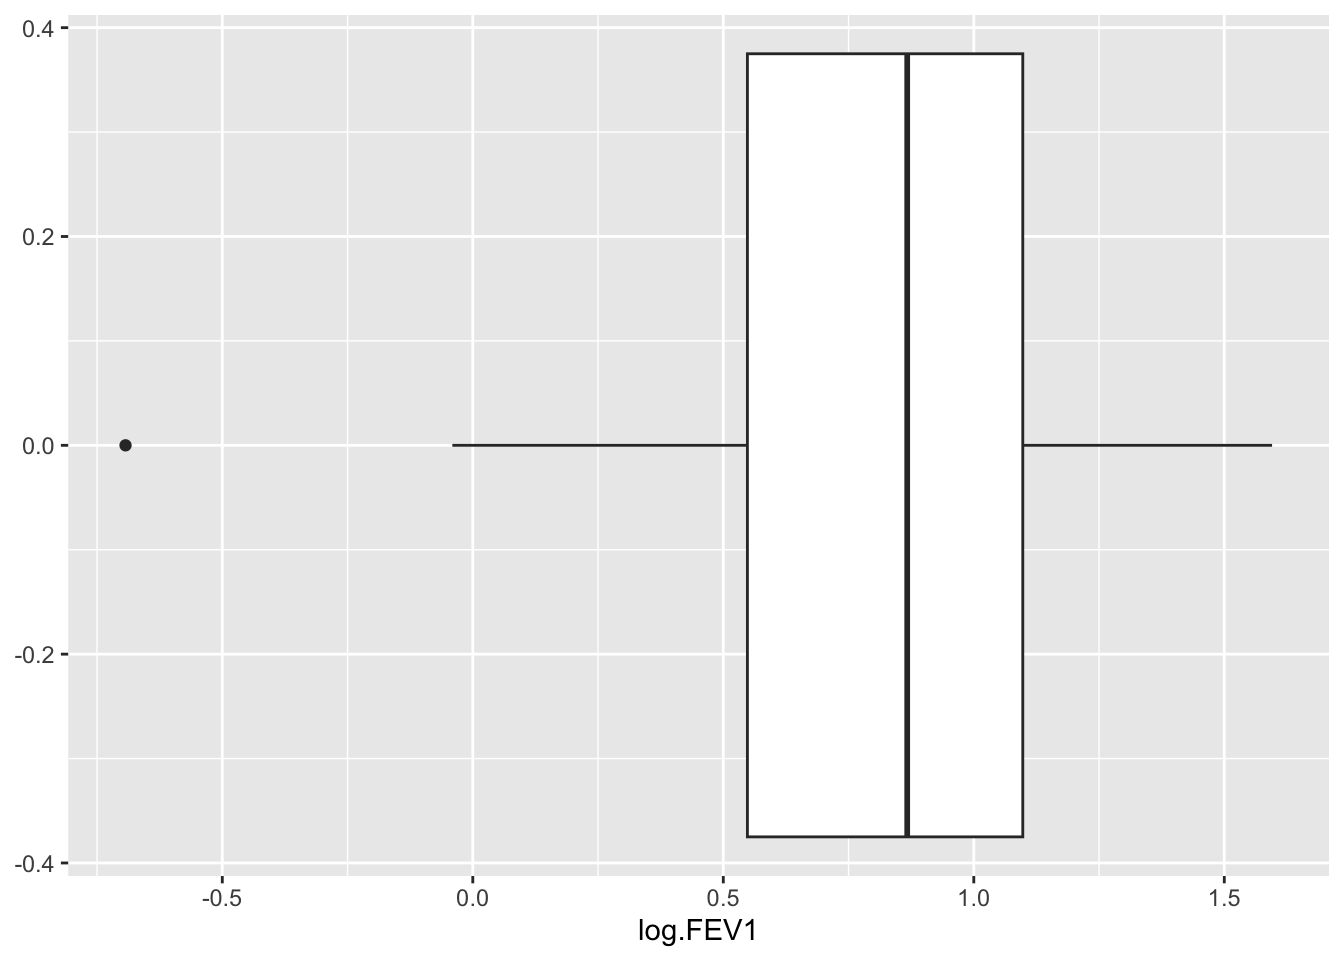
\includegraphics{HW1_files/figure-latex/chunk_Q2a-1.pdf}

\begin{Shaded}
\begin{Highlighting}[]
\CommentTok{\# spaghetti plot}
\FunctionTok{ggplot}\NormalTok{(topeka, }\FunctionTok{aes}\NormalTok{(}\AttributeTok{x =}\NormalTok{ age, }\AttributeTok{y =}\NormalTok{ log.FEV1, }\AttributeTok{group =}\NormalTok{ id, }\AttributeTok{color =}\NormalTok{ id)) }\SpecialCharTok{+} 
  \FunctionTok{geom\_line}\NormalTok{() }\SpecialCharTok{+} 
  \FunctionTok{scale\_x\_continuous}\NormalTok{(}\AttributeTok{breaks =} \FunctionTok{c}\NormalTok{(}\DecValTok{5}\NormalTok{, }\DecValTok{10}\NormalTok{, }\DecValTok{15}\NormalTok{, }\DecValTok{20}\NormalTok{)) }\SpecialCharTok{+}
  \FunctionTok{scale\_y\_continuous}\NormalTok{(}\AttributeTok{limits =} \FunctionTok{c}\NormalTok{(}\SpecialCharTok{{-}}\FloatTok{0.25}\NormalTok{, }\FloatTok{1.5}\NormalTok{))}
\end{Highlighting}
\end{Shaded}

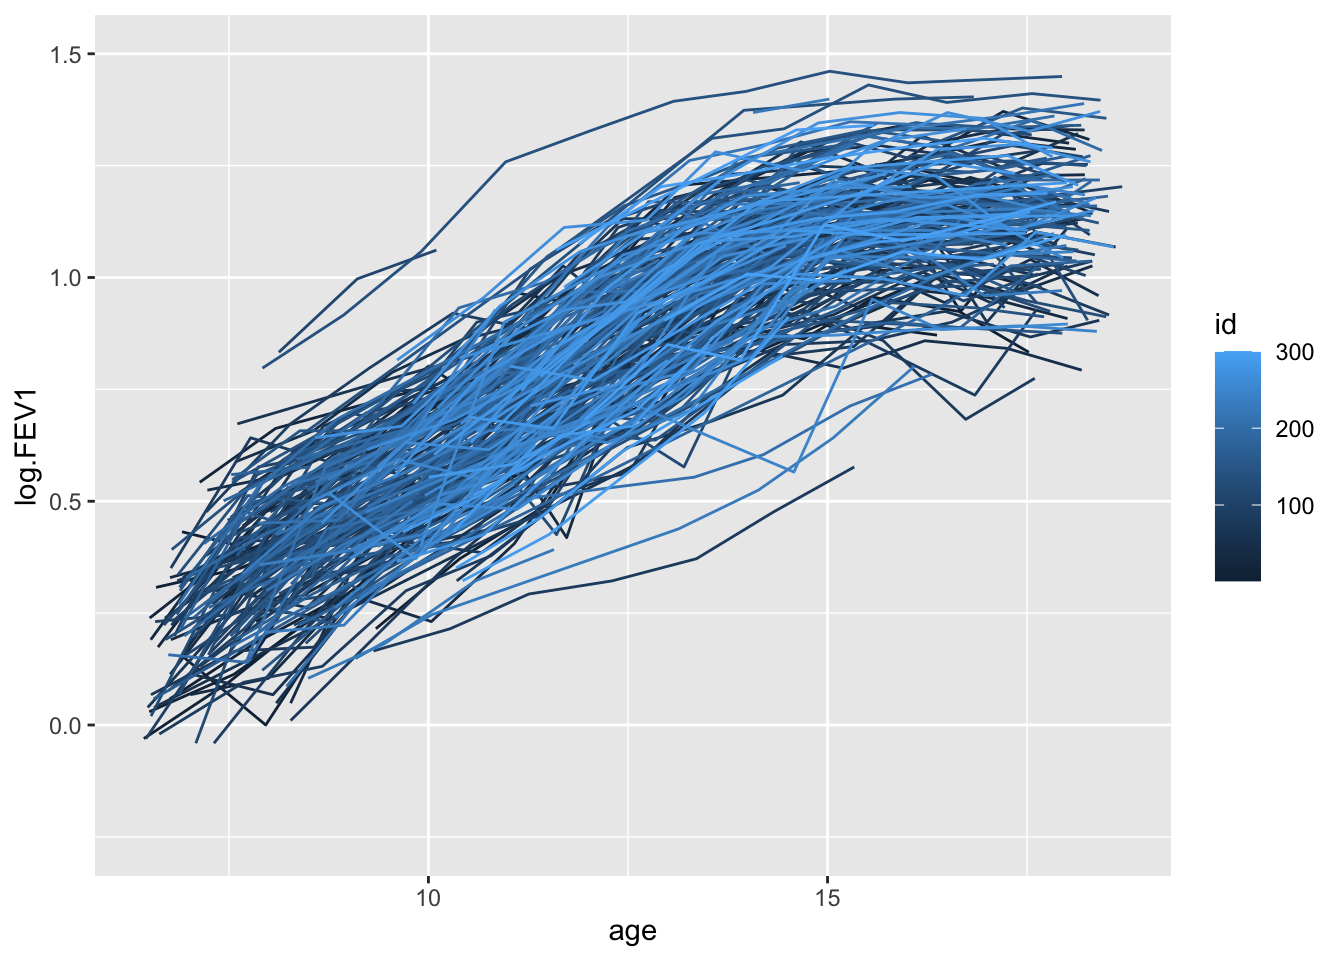
\includegraphics{HW1_files/figure-latex/chunk_Q2a-2.pdf}

\begin{Shaded}
\begin{Highlighting}[]
\CommentTok{\# dependence}
\FunctionTok{pairs}\NormalTok{(topeka)}
\end{Highlighting}
\end{Shaded}

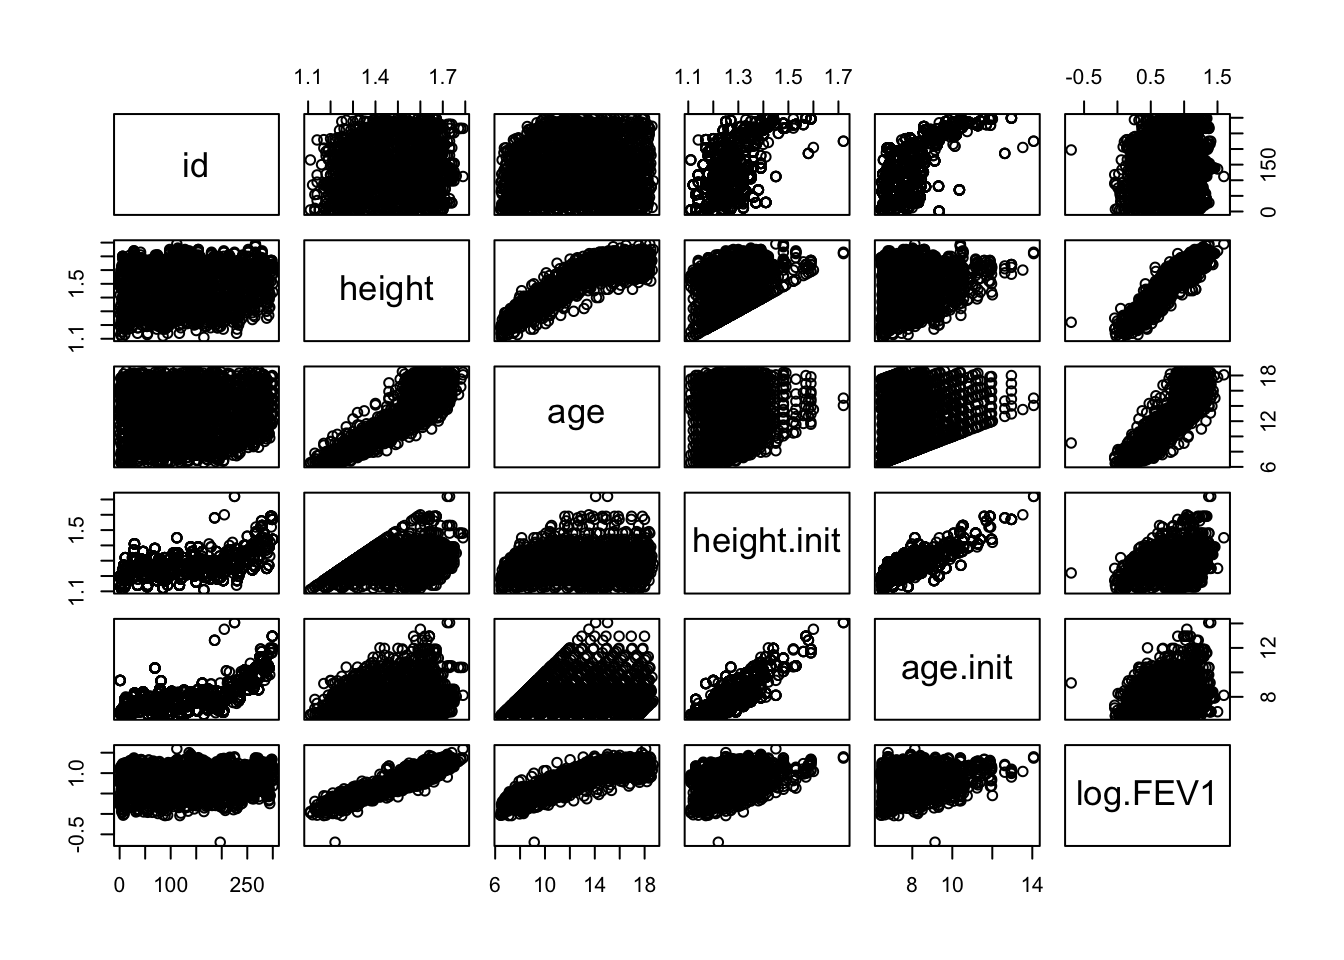
\includegraphics{HW1_files/figure-latex/chunk_Q2a-3.pdf}

\begin{Shaded}
\begin{Highlighting}[]
\NormalTok{corrplot}\SpecialCharTok{::}\FunctionTok{corrplot}\NormalTok{(}\FunctionTok{cor}\NormalTok{(topeka[]))}
\end{Highlighting}
\end{Shaded}

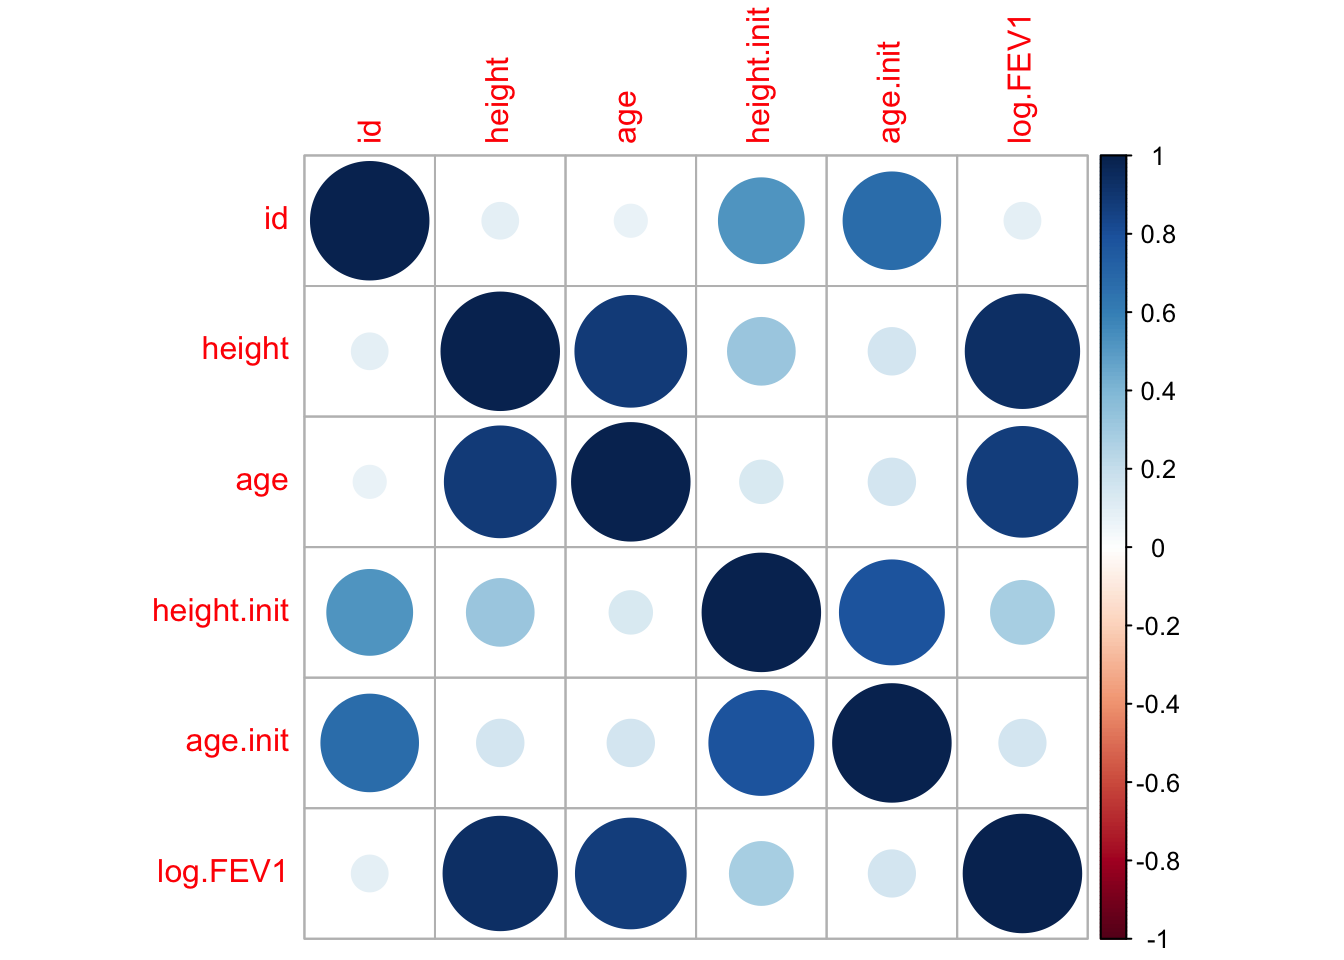
\includegraphics{HW1_files/figure-latex/chunk_Q2a-4.pdf}

There are 5 variables and 1 outcome in the topeka dataset, which
consists of 300 clusters with 1994 measurements. Number of measurements
within each cluster ranges from 1 to 12, with mean being 6.6 and median
being 7. The mean age of the subjects upon their recruitment was 8.03,
while the height was 1.28m. For simplicity, the age and height variables
could be standardized when conducting the longitudal analysis. One
outlier of the outcome log.FEV1 was observed which should be further
investigated. In the correlation plot one can see that the covariates
age and height are highly correlated, indicating they might be dependent
of each other.

\end{document}
